\questionheader{ex:s1.9}

\noindent 
Recall that we are using $\log x$ to denote the logarithm of $x$ with
base $e$. In other courses it is often denoted $\ln x$.


%%%%%%%%%%%%%%%%%%
\subsection*{\Conceptual}
%%%%%%%%%%%%%%%%%%



\begin{Mquestion}[2015A]\label{prob:s1.9_1}
For each of the following integrals, choose the substitution that
is most beneficial for evaluating the integral.
\begin{enumerate}[(a)]
\item
$\displaystyle \int \frac{2x^2}{\sqrt{9x^2-16}} \, \dee{x}$ 

\item $\displaystyle \int \frac{x^4-3}{\sqrt{1-4x^2}} \, \dee{x}$ 

\item $\displaystyle \int {(25+x^2)}^{-5/2} \, \dee{x}$
\end{enumerate}


\end{Mquestion}

\begin{hint} 
The beginning of this section has a template for choosing a substitution. Your goal is to use a trig identity to turn the argument of the square root into a perfect square, so you can cancel $\sqrt{(\mbox{something})^2}=|\mbox{something}|$. 
\end{hint}

\begin{answer} 
(a) $x=\dfrac{4}{3}\sec\theta$
\qquad (b) $x=\dfrac{1}{2}\sin\theta$
\qquad (c) $x=5\tan\theta$
\end{answer}

\begin{solution} 
In the text, there is a template for choosing an appropriate substitution, but for this problem we will explain the logic of the choices.

The trig identities that we can use are:
\begin{align*}
&1-\sin^2\theta=\cos^2\theta & &\tan^2 \theta +1 = \sec^2 \theta & &\sec^2 \theta - 1 =\tan^2 \theta
\intertext{They have the following forms:}
&\mbox{constant } - \mbox{ function} &&\mbox{function } + \mbox{ constant} & 
&\mbox{function } - \mbox{ constant} 
\end{align*}
In order to cancel out the square root, we should choose a substitution that will match the argument under the square root with the trig identity of the corresponding form. 

(a)
There's not an obvious non-trig substitution for evaluating this problem, so we want a trigonometric substitution to get rid of the square root in the denominator. Under the square root is the function $9x^2-16$, which has the form (function) $-$ (constant). This form matches the trig identity $\sec^2 \theta - 1 = \tan^2 \theta$. We can set $x$ to be whatever we need it to be, but we don't have the same control over the constant, 16. So, to make the substitution work, we use a different form of the trig identity: multiplying both sides  by 16, we get
\begin{align*}
~16\sec^2\theta - 16 &= 16\tan^2\theta
\intertext{What we want is a substitution that gives us}
9x^2-16&=16\sec^2\theta - 16\\
\mbox{So,}\qquad 9x^2&=16\sec^2\theta\\
x &= \frac{4}{3}\sec\theta
\intertext{Using this substitution,}
\sqrt{9x^2-16}&=\sqrt{16\sec^2\theta-16}\\
&=\sqrt{16\tan^2\theta}\\
&=4|\tan\theta|
\end{align*}
So, we eliminated the square root.

\noindent (b)
There's not an obvious non-trig substitution for evaluating this problem, so we want a trigonometric substitution to get rid of the square root in the denominator. Under the square root is the function $1-4x^2$, which has the form (constant) $-$ (function). This form matches the trig identity $1-\sin^2\theta = \cos^2\theta$. What we want is a substitution that gives us
\begin{align*}
1-4x^2&=1-\sin^2\theta\\
\mbox{So,}\qquad 4x^2&=\sin^2\theta\\
x &= \frac{1}{2}\sin\theta
\intertext{Using this substitution,}
\sqrt{1-4x^2}&=\sqrt{1-\sin^2\theta}\\
&=\sqrt{\cos^2\theta}\\
&=|\cos\theta|
\end{align*}
So, we eliminated the square root. We remark that the absolute value signs are not needed in $|\cos\theta|$, because, for $-\frac{1}{2}\le x\le\frac{1}{2}$,
we have $\theta=\arcsin(2x)$ between $-\frac{\pi}{2}$ and $\frac{\pi}{2}$,
and $\cos(\theta)\ge 0$ for those $\theta$'s.


\noindent (c)
There's not an obvious non-trig substitution for evaluating this problem, so we want a trigonometric substitution to get rid of the fractional power. (That is, we want to eliminate the square root.) The function under the power is $25+x^2$, which has the form (constant) $+$ (function). This form matches the trig identity $\tan^2 \theta + 1 = \sec^2 \theta$. We can set $x$ to be whatever we need it to be, but we don't have the same control over the constant, 25. So, to make the substitution work, we use a different form of the trig identity: multiplying both sides  by 25, we get
\begin{align*}
25\tan^2 \theta + 25 &= 25\sec^2 \theta
\intertext{What we want is a substitution that gives us}
25+x^2&=25\tan^2\theta+25\\
\mbox{So,}\qquad x^2&=25\tan^2\theta\\
x &= 5\tan\theta
\intertext{Using this substitution,}
(25+x^2)^{-5/2}&=(25+25\tan^2\theta)^{-5/2}\\
&=(25\sec^2\theta)^{-5/2}\\
&=(5|\sec\theta|)^{-5}
\end{align*}
So, we eliminated the square root. We remark that the absolute value signs are not needed in $|\sec\theta|$, because, for $-\infty< x<\infty$,
we have $\theta=\arctan(x/5)$ between $-\frac{\pi}{2}$ and $\frac{\pi}{2}$,
and $\sec(\theta)\ge 0$ for those $\theta$'s.
\end{solution}
%%%%%%%%%%%%%%%%%%%
\begin{Mquestion}\label{prob_21.9:complete}
For each of the following integrals, choose a trigonometric substitution that
will eliminate the roots.
\begin{enumerate}[(a)]
\item $\displaystyle\int \dfrac{1}{\sqrt{x^2-4x+1}}~\dee{x}$
\item $\displaystyle\int \dfrac{(x-1)^6}{(-x^2+2x+4)^{3/2}}~\dee{x}$
\item $\displaystyle\int \dfrac{1}{\sqrt{4x^2+6x+10}}~\dee{x}$
\item $\displaystyle\int \sqrt{x^2-x}~\dee{x}$
\end{enumerate}
\end{Mquestion}
\begin{hint}
You want to do the same thing you did in Question~\ref{prob:s1.9_1}, but you'll have to complete the square first.
\end{hint}
\begin{answer}
(a) $x-2=\sqrt{3}\sec u$\qquad
(b) $x-1=\sqrt{5}\sin u$
\qquad
(c) $\left(2x+\dfrac{3}{2}\right) =\dfrac{\sqrt{31}}{2}\tan u$
\\
(d) $x - \dfrac{1}{2}=\dfrac{1}{2}\sec u$\qquad 
\end{answer}
\begin{solution}
Just as in Question~\ref{prob:s1.9_1}, we want to choose a trigonometric substitution that will allow us to eliminate the square roots. Before we can make that choice, though, we need to complete the square. In subsequent problems, we won't show the algebra behind completing the square, but for this problem we'll work it out explicitly. After some practice, you'll  be able to do this step in your head for many cases.

After the squares are completed, the choice of trig substitution follows the logic outlined in the solutions to Question~\ref{prob:s1.9_1}, or (equivalently) the template in the text.

\begin{enumerate}[(a)]
\item
The quadratic function under the square root is $x^2-4x+1$. To complete the square, we match the non-constant terms to those of a perfect square.
\begin{align*}
(ax+b)^2&=a^2x^2+2abx+b^2\\
\textcolor{red}{x^2}-\textcolor{blue}{4x}+1&=\textcolor{red}{a^2x^2} + \textcolor{blue}{2abx} +b^2 + c \quad\mbox{for some constant $c$}
\end{align*}
\begin{itemize}
\item \textcolor{red}{Looking at the leading term tells us $a=1$. }
\item \textcolor{blue}{Then the second term tells us $-4=2ab=2b$, so $b=-2$.}
\item Finally, the constant terms give us $1=b^2+c=4+c$, so $c=-3$.
\end{itemize}

 \[\displaystyle\int \dfrac{1}{\sqrt{x^2-4x+1}}~\dee{x}=\displaystyle\int \dfrac{1}{\sqrt{(x-2)^2-3}}~\dee{x}=\displaystyle\int \dfrac{1}{\sqrt{\left(x-2\vphantom{\sqrt{3}}\right)^2-\sqrt{3}^2}}~\dee{x}\]
 
So we use the substitution $(x-2) = \sqrt{3}\sec u$, which eliminates the square root:
\[\sqrt{\left(x-2\right)^2-3}=\sqrt{3\sec^2 u - 3} = \sqrt{3\tan^2 u} = \sqrt{3}|\tan u|\]
%
\item 
The quadratic function under the square root is $-x^2+2x+4=-[x^2-2x-4]$. To complete the square, we match the non-constant terms to those of a perfect square. We factored out the negative to make things a little easier--don't forget to put it back in before choosing a substitution!
\begin{align*}
(ax+b)^2&=a^2x^2+2abx+b^2\\
\textcolor{red}{x^2}-\textcolor{blue}{2x}-4&=\textcolor{red}{a^2x^2} + \textcolor{blue}{2abx} +b^2 + c \quad\mbox{for some constant $c$}
\end{align*}
\begin{itemize}
\item \textcolor{red}{Looking at the leading term tells us $a=1$. }
\item \textcolor{blue}{Then the second term tells us $-2=2ab=2b$, so $b=-1$.}
\item Finally, the constant terms give us $-4=b^2+c=1+c$, so $c=-5$.
\item Then $-x^2+2x+4 = -[x^2-2x-4]=-[(x-1)^2-5]=5-(x-1)^2$.
\end{itemize}

\[\displaystyle\int \dfrac{(x-1)^6}{(-x^2+2x+4)^{3/2}}~\dee{x}=\displaystyle\int \dfrac{(x-1)^6}{(5-(x-1)^2)^{3/2}}~\dee{x}=\displaystyle\int \dfrac{(x-1)^6}{\left(\sqrt{5}^2-\left(x-1\vphantom{\sqrt{3}}\right)^2\right)^{3/2}}~\dee{x}\]
So we use the substitution $(x-1) = \sqrt{5}\sin u$, which eliminates the square root (fractional power):
\[(5-\left(x-1\right)^2)^{3/2}=\left(5-5\sin^2u\right)^{3/2} = \left(5\cos^2 u\right)^{3/2} = 5\sqrt{5}|\cos^3 u|\]
%
\item 
The quadratic function under the square root is $4x^2+6x+10$. To complete the square, we match the non-constant terms to those of a perfect square.
\begin{align*}
(ax+b)^2&=a^2x^2+2abx+b^2\\
\textcolor{red}{4x^2}+\textcolor{blue}{6x}+10&=\textcolor{red}{a^2x^2} + \textcolor{blue}{2abx} +b^2 + c \quad\mbox{for some constant $c$}
\end{align*}
\begin{itemize}
\item \textcolor{red}{Looking at the leading term tells us $a=2$. }
\item \textcolor{blue}{Then the second term tells us $6=2ab=4b$, so $b=\frac{3}{2}$.}
\item Finally, the constant terms give us $10=b^2+c=\frac{9}{4}+c$, so $c=\frac{31}{4}$.
\end{itemize}
\[\displaystyle\int \dfrac{1}{\sqrt{4x^2+6x+10}}~\dee{x}=\displaystyle\int \dfrac{1}{\sqrt{\left(2x+\frac{3}{2}\right)^2+\frac{31}{4}}}~\dee{x}
=\displaystyle\int \dfrac{1}{\sqrt{\left(2x+\frac{3}{2}\right)^2+\left(\frac{\sqrt{31}}{2}\right)^2}}~\dee{x}\]
So we use the substitution $\left(2x+\frac{3}{2}\right) =\frac{\sqrt{31}}{2}\tan u$, which eliminates the square root:
\[\sqrt{\left(2x+\frac{3}{2}\right)^2+\frac{31}{4}}=\sqrt{\frac{31}{4}\tan^2 u +\frac{31}{4}} = \sqrt{\frac{31}{4}\sec^2 u} =\frac{\sqrt{31}}{2}|\sec u|\]
%
\item 
The quadratic function under the square root is $x^2-x$. To complete the square, we match the non-constant terms to those of a perfect square.
\begin{align*}
(ax+b)^2&=a^2x^2+2abx+b^2\\
\textcolor{red}{x^2}-\textcolor{blue}{x}&=\textcolor{red}{a^2x^2} + \textcolor{blue}{2abx} +b^2 + c \quad\mbox{for some constant $c$}
\end{align*}
\begin{itemize}
\item \textcolor{red}{Looking at the leading term tells us $a=1$. }
\item \textcolor{blue}{Then the second term tells us $-1=2ab=2b$, so $b=-\frac{1}{2}$.}
\item Finally, the constant terms give us $0=b^2+c=\frac{1}{4}+c$, so $c=-\frac{1}{4}$.
\end{itemize}


\[\displaystyle\int \sqrt{x^2-x}~\dee{x}=\displaystyle\int \sqrt{\left(x-\frac{1}{2}\right)^2 -\frac{1}{4}}~\dee{x}=\displaystyle\int  \sqrt{\left(x-\frac{1}{2}\right)^2 -\left(\frac{1}{2}\right)^2}~\dee{x}\]
So we use the substitution $(x-1/2) = \frac{1}{2}\sec u$, which eliminates the square root:
\[\sqrt{\left(x-\frac{1}{2}\right)^2-\frac{1}{4}}=\sqrt{\frac{1}{4}{\sec\vphantom{|}}^2 u - \frac{1}{4}} = \sqrt{\frac{1}{4}\tan^2 u} =\frac{1}{2}|\tan u|\]

\end{enumerate}

\end{solution}
%%%%%%%%%%%%%%%%%%%



\begin{question}\label{prob:s1.9_3}
In each part of this question, assume  $\theta$ is an angle in the interval $\left[ 0,\pi/2\right]$.
\begin{enumerate}[(a)]
\item If $\sin\theta=\dfrac{1}{20}$, what is $\cos\theta$~?
\item If $\tan\theta=7$, what is $\csc\theta$~?
\item If $\sec\theta=\dfrac{\sqrt{x-1}}{2}$, what is $\tan\theta$~?
\end{enumerate}
\end{question}
\begin{hint}
Since $\theta$ is acute, you can draw it as an angle of a right triangle. The given information will let you label two sides of the triangle, and the Pythagorean Theorem will lead you to the third.
\end{hint}
\begin{answer}
(a) $\dfrac{\sqrt{399}}{20}$\qquad
(b) $\dfrac{5\sqrt{2}}{7}$\qquad
(c) $\dfrac{\sqrt{x-5}}{2} $
\end{answer}
\begin{solution}
\begin{enumerate}[(a)]
\item If $\sin\theta=\dfrac{1}{20}$ and $\theta$ is between 0 and $\pi/2$, then we can draw a right triangle with angle $\theta$ that has opposite side length 1, and hypotenuse length 20. By the Pythagorean Theorem, the adjacent side has length $\sqrt{20^2-1^2}=\sqrt{399}$. So,  $\cos\theta = \dfrac{\mathrm{adj}}{\mathrm{hyp}}=\dfrac{\sqrt{399}}{20}$.
\begin{center}
\trigtri{\theta}{\sqrt{399}}{1}{20}
\end{center}
We can do a quick ``reasonableness" check here: $\frac{1}{20}$ is pretty close to 0, so we might expect $\theta$ to be pretty close to 0, and so $\cos \theta$ should be pretty close to 1. Indeed it is: $\dfrac{\sqrt{399}}{20}\approx \dfrac{\sqrt{400}}{20}=\dfrac{20}{20}=1$.

Alternately, we can solve this problem using identities.
\begin{align*}
\sin^2 \theta + \cos^2 \theta &=1\\
\left(\frac{1}{20}\right)^2+ \cos^2 \theta &=1\\
\cos\theta &= \pm\sqrt{1-\frac{1}{400}}=\pm\frac{\sqrt{399}}{20}
\intertext{Since $0 \leq \theta \leq \frac{\pi}{2}$, $\cos\theta \geq 0$, so}
\cos\theta &= \frac{\sqrt{399}}{20}
\end{align*}
\item If $\tan\theta=7$ and $\theta$ is between 0 and $\pi/2$, then we can draw a right triangle with angle $\theta$ that has opposite side length 7 and adjacent side length 1. By the Pythagorean Theorem, the hypotenuse has length $\sqrt{7^2+1^2} = \sqrt{50}=5\sqrt{2}$. So,  $\csc\theta = \dfrac{\mathrm{hyp}}{\mathrm{opp}}=\dfrac{5\sqrt{2}}{7}$.
\begin{center}
\trigtri{\theta}{1}{7}{5\sqrt{2}}
\end{center}

Again, we can do a quick reasonableness check. Since 7 is much larger than 1, the triangle we're thinking of doesn't look much like the triangle in our standardized picture above: it's really quite tall, with a small base. So, the opposite side and hypotenuse are pretty close in length. Indeed, $\dfrac{5\sqrt{2}}{7}\approx 7.071$, so this dimension seems reasonable.

\item If $\sec\theta=\dfrac{\sqrt{x-1}}{2}$ and $\theta$ is between 0 and $\pi/2$, then we can draw a right triangle with angle $\theta$ that has hypotenuse length $\sqrt{x-1}$ and adjacent side length 2. By the Pythagorean Theorem, the opposite side has length $\sqrt{\sqrt{x-1}^2 - 2^2} = \sqrt{x-1-4}=\sqrt{x-5}$. So,  $\tan\theta = \dfrac{\mathrm{opp}}{\mathrm{adj}}=\dfrac{\sqrt{x-5}}{2}$.
\begin{center}
\trigtri{\theta}{2}{\sqrt{x-5}}{\sqrt{x-1}}
\end{center}

We can also solve this using identities. Note that since $\sec\theta$ exists,  $\theta \neq \frac{\pi}{2}$.
\begin{align*}
\tan^2\theta+1&=\sec^2\theta\\
\tan^2\theta+1&=\left(\frac{\sqrt{x-1}}{2}\right)^2=\frac{x-1}{4}\\
\tan\theta &= \pm\sqrt{\frac{x-1}{4}-1} = \pm\frac{\sqrt{x-5}}{2}
\intertext{Since $0 \leq \theta < \frac{\pi}{2}$, $\tan\theta \geq 0$, so}
\tan\theta &= \frac{\sqrt{x-5}}{2}
\end{align*}
\end{enumerate}

\end{solution}
%%%%%%%%%%%%%%%%%%%



\begin{Mquestion}\label{prob:s1.9_4}
Simplify the following expressions.
\begin{enumerate}[(a)]
\item $\sin\left(\arccos \left(\frac{x}{2}\right)\right)$
\item $\sin\left(\arctan \left(\frac{1}{\sqrt{3}}\right)\right)$
\item $\sec\left(\arcsin \left(\sqrt{x}\right)\right)$
\end{enumerate}
\end{Mquestion}
\begin{hint}
You can draw a right triangle with angle $\theta$, and use the given information to label two of the sides. The Pythagorean Theorem gives you the third side.
\end{hint}
\begin{answer}
(a) $\dfrac{\sqrt{4-x^2}}{2}$\qquad
(b) $\dfrac{1}{2}$\qquad
(c) $\dfrac{1}{\sqrt{1-x}}$
\end{answer}
\begin{solution}
\begin{enumerate}[(a)]
\item Let $\theta = \arccos \left(\frac{x}{2}\right)$. That is, $\cos(\theta) = \frac{x}{2}$, and $0 \leq \theta \leq \pi$. Then we can draw the corresponding right triangle with angle $\theta$ with adjacent side of signed length $x$ (we note that if $\theta > \frac{\pi}{2}$, then $x$ is negative) and hypotenuse of length $2$. By the Pythagorean Theorem, the opposite side of the triangle has length $\sqrt{4-x^2}$.
\begin{center}
\trigtri{\theta}{x}{\sqrt{4-x^2}}{2}
\end{center}
So,

\[\sin\left(\arccos \left(\frac{x}{2}\right)\right)=\sin \theta = \frac{\mathrm{opp}}{\mathrm{hyp}} = \frac{\sqrt{4-x^2}}{2}\]


\item Let $\theta = \arctan \left(\frac{1}{\sqrt{3}}\right)$. That is, $\tan(\theta) = \frac{1}{\sqrt{3}}$, and $-\frac{\pi}{2} \leq \theta \leq \frac{\pi}{2}$. 

\begin{description}
\item[Solution 1:] Then $\theta = \dfrac{\pi}{6}$, so $\sin\theta = \dfrac{1}{2}$.
\item[Solution 2:] 
Then we can draw the corresponding right triangle with angle $\theta$ with opposite side of length $1$  and adjacent side of length $\sqrt{3}$. By the Pythagorean Theorem, the hypotenuse of the triangle has length $\sqrt{\sqrt{3}^2+1^2}=2$.
\begin{center}
\trigtri{\theta}{\sqrt{3}}{1}{2}
\end{center}
So,

\[\sin\left(\arctan \left(\frac{1}{\sqrt{3}}\right)\right)=\sin \theta = \frac{\mathrm{opp}}{\mathrm{hyp}} = \frac{1}{2}\]
\end{description}

\item Let $\theta = \arcsin \left(\sqrt{x}\right)$. That is, $\sin(\theta) = \sqrt{x}$, and $-\frac{\pi}{2} \leq \theta \leq \frac{\pi}{2}$. Then we can draw the corresponding right triangle with angle $\theta$ with opposite side of length $\sqrt{x}$ and hypotenuse of length $1$. By the Pythagorean Theorem, the adjacent side of the triangle has length $\sqrt{1-x}$.
\begin{center}
\trigtri{\theta}{\sqrt{1-x}}{\sqrt{x}}{1}
\end{center}
So,

\[\sec\left(\arcsin \left(\sqrt{x}\right)\right)=\sec \theta = \frac{\mathrm{hyp}}{\mathrm{adj}} = \frac{1}{\sqrt{1-x}}\]

\end{enumerate}

\end{solution}
%%%%%%%%%%%%%%%%%%%



%%%%%%%%%%%%%%%%%%
\subsection*{\Procedural}
%%%%%%%%%%%%%%%%%%

\begin{question}[2016Q4]\label{prob:s1.9_P1}
Evaluate $\displaystyle\int \frac1{(x^2+4)^{3/2}} \,\dee{x}.$
\end{question}

\begin{hint} 
As in Question \ref{prob:s1.9_1}, choose an appropriate substitution. Your answer should be in terms of your original variable, $x$, which can be achieved using the methods of Question~\ref{prob:s1.9_3}.
\end{hint}

\begin{answer} 
$\dfrac14\cdot \dfrac x{\sqrt{x^2+4}} + C$
\end{answer}

\begin{solution} 
Let $x = 2\tan\theta$, so that $x^2+4 = 4\tan^2\theta+4=4\sec^2\theta$ and $\dee{x} = 2\sec^2\theta\,\dee{\theta}$. Then
\begin{align*}
\int \frac1{(x^2+4)^{3/2}} \,\dee{x} &= \int \frac1{(4\sec^2\theta)^{3/2}} \cdot 2\sec^2\theta\,\dee{\theta} \\
&= \int \frac{2\sec^2\theta}{8\sec^3\theta} \,\dee{\theta} \\
&=\frac14 \int \cos\theta\,\dee{\theta} \\
&= \frac14\sin\theta+C = \frac14 \frac x{\sqrt{x^2+4}} + C
\qquad\qquad\smash{
\trigtri{\theta}{2}{x}{\sqrt{x^2+4}}}
\end{align*}
To find $\sin\theta$ in terms of $x$, we construct the right triangle above.
Since $\tan\theta = \dfrac{x}{2} = \dfrac{\mbox{opp}}{\mbox{adj}}$, we label the opposite side $x$ and the adjacent side $2$. By the Pythagorean Theorem, the hypotenuse has length $\sqrt{x^2+4}$. Then $\sin\theta = \dfrac{\mbox{opp}}{\mbox{hyp}} = \dfrac{x}{\sqrt{x^2+4}}$. 

To see why we could write $(\sec^2\theta)^{3/2} =\sec^3\theta$, as opposed to 
$(\sec^2\theta)^{3/2} =\big|\sec^3\theta\big|$, in the second line above, see
Example \eref{CLP101}{eg:INVTRIGb} in the CLP-2 text.

As a check, we observe that the derivative of the answer
\begin{align*}
\diff{}{x} \left(\frac14 \frac x{\sqrt{x^2+4}} +C\right)
&=\frac14\frac 1{\sqrt{x^2+4}} - \frac{1}{2\times 4}\frac{x(2x)}{{\big(x^2+4\big)}^{3/2}}
=\frac{\frac{x^2}{4}+1-\frac{x^2}{4}}{{\big(x^2+4\big)}^{3/2}} \\
&=\frac{1}{{\big(x^2+4\big)}^{3/2}} 
\end{align*}
is exactly the integrand.
\end{solution}
%%%%%%%%%%%%%%%%%%%

\begin{question}[2016Q4]
Evaluate
$\displaystyle\int_0^4 \frac{1}{{(4+x^2)}^{3/2}}\,\dee{x}$. 
Your answer may not contain inverse trigonometric functions.
\end{question}
\begin{hint} 
As in Question \ref{prob:s1.9_1}, choose an appropriate substitution. Your answer will be a number, so as long as you change your limits of integration when you substitute, you don't need to bother changing the antiderivative back into the original variable $x$. However, you might want to use the techniques of Question~\ref{prob:s1.9_4} to simplify your final answer.
\end{hint}

\begin{answer} 
$ \dfrac{1}{2\sqrt{5}}$
\end{answer}

\begin{solution} 
\begin{description}
\item[Solution 1:]
As in Question~\ref{prob:s1.9_P1}, substitute $x=2\tan u$,  $\dee{x}=2 \sec^2u\,\dee{u}$. Note that when $x=4$
we have $4=2\tan u$, so that $\tan u=2$.
\begin{align*}
\int_0^4 \frac{1}{{(4+x^2)}^{3/2}}\,\dee{x}
&=\int_0^{\arctan 2} \frac{1}{{(4+4\tan^2 u)}^{3/2}}\,2\sec^2 u\,\dee{u}
   \\[0.1in]
&=\int_0^{\arctan 2} \frac{2\sec^2 u}{{(2\sec u)}^{3}}\,\dee{u}
   \\[0.1in]
&=\frac{1}{4}\int_0^{\arctan 2} \frac{\sec^2u}{\sec^3u}\,\dee{u}\\[0.1in]
&=\frac{1}{4}\int_0^{\arctan 2} \cos u\,\dee{u}
\qquad\qquad\smash{\raisebox{-0.1\height}{
%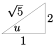
\includegraphics{fig/OQ16_4_4}
\trigtri{u}{1}{2}{\sqrt{5}}
}}
\\
&=\bigg[\frac{1}{4}\sin u \bigg]_0^{\arctan2}
\\
&=\frac{1}{4} \big( \sin(\arctan 2) - 0 \big)
= \frac{1}{2\sqrt{5}}
\end{align*}
To find $\sin(\arctan 2)$, we use the right triangle above, with angle $u=\arctan 2$. Since $\tan u=2 = \dfrac{\mbox{opp}}{\mbox{adj}}$, we label the opposite side as 2, and the adjacent side as 1. The Pythagorean Theorem tells us the hypotenuse has length $\sqrt{5}$, so \smash{$\sin u = \dfrac{\mbox{opp}}{\mbox{hyp}} = \dfrac{2}{\sqrt{5}}$.}

\item[Solution 2:]
Using our result from Question~\ref{prob:s1.9_P1},
\begin{align*}
\int_0^4 \frac{1}{{(4+x^2)}^{3/2}}\,\dee{x}&=\frac{1}{4}\left[ \dfrac x{\sqrt{x^2+4}}\right]_0^4\\
&=\frac{1}{4}\cdot \dfrac{4}{\sqrt{4^2+4}}=\frac{1}{2\sqrt{5}}
\end{align*}
\end{description}
\end{solution}
%%%%%%%%%%%%%%%%%%%


\begin{Mquestion}[M105 2013A]
Evaluate $\displaystyle\int_0^{5/2} \frac{\dee{x}}{\sqrt{25-x^2}}$.
\end{Mquestion}

\begin{hint} 
Question \ref{prob:s1.9_1} guides the way to finding the appropriate substitution.
Since the integral is definite, your final answer will be a number. Your limits of integration should be common reference angles.
\end{hint}

\begin{answer} 
$\dfrac{\pi}{6}$ 
\end{answer}

\begin{solution} 
 Make the change of variables $x=5\sin\theta$, $\dee{x}=5\cos\theta\,\dee{\theta}$. 
Since $x=0$ corresponds to $\theta=0$ and $x=\frac{5}{2}$ correponds to
$\sin\theta=\half$ or $\theta =\frac{\pi}{6}$,
\begin{align*}
\int_0^{5/2} \frac{\dee{x}}{\sqrt{25-x^2}}
=\int_0^{\pi/6} \frac{5\cos\theta\,\dee{\theta}}{\sqrt{25-25\sin^2\theta}}
=\int_0^{\pi/6} \dee{\theta}
=\frac{\pi}{6}
\end{align*}
\end{solution}
%%%%%%%%%%%%%%%%%%%

\begin{Mquestion}[M105 2015A]
Evaluate $\displaystyle\int \frac{\dee{x}}{\sqrt{x^2+25}}$.
You may use that 
${\displaystyle\int} \sec x\ \dee{x} = \log\big|\sec x+\tan x\big|+C$.
\end{Mquestion}

\begin{hint} 
Question \ref{prob:s1.9_1} guides the way to finding the appropriate substitution. Since you have in indefinite integral, make sure to get your answer back in terms of the original variable, $x$. Question \ref{prob:s1.9_3} gives a reliable method for this.
\end{hint}

\begin{answer} 
$\displaystyle\log\left|\sqrt{1+\frac{x^2}{25}}+\frac{x}{5}\right|+C$
\end{answer}

\begin{solution} 
Substitute $x=5\tan u$, so that $\dee{x}=5 \sec^2u\,\dee{u}$.
\begin{align*}
\int\frac{1}{\sqrt{x^2+25}}\,\dee{x}
&=\int \frac{1}{\sqrt{25\tan^2 u+25}}\,5\sec^2 u\,\dee{u}   \\[0.1in]
&=\int \frac{5\sec^2u}{5\sec u}\,\dee{u}
=\int \sec u\,\dee{u} \\[0.1in]
&= \log\big|\sec u+\tan u\big|+C
\qquad\qquad\smash{
\trigtri{u}{5}{x}{\sqrt{x^2+25}}} \\
&= \log\Big|\sqrt{1+\frac{x^2}{25}}+\frac{x}{5}\Big|+C
\end{align*}
To find $\sec u$ and $\tan u$, we have two options. One is to set up a right triangle with angle $u$ and $\tan u = \frac{x}{5}$. Then we can label the opposite side $x$ and the adjacent side 5, and use Pythagoras to find that the hypotenuse is $\sqrt{x^2+25}$.

Another option is to look back at our work a little more closely--in fact, we've already found what we're looking for. Since we used the substitution $x=5\tan u$, this gives us $\tan u = \frac{x}{5}$. In the denominator of the integrand, we simplified $\sqrt{x^2+25} = 5\sec u$, so $\sec u = \frac{1}{5}\sqrt{x^2+25} = \sqrt{1+\frac{x^2}{25}}$.

To see why we could write $\sqrt{x^2+25} =5\sec u$, as opposed to 
$\sqrt{x^2+25} =5|\sec u|$,  see
Example \eref{CLP101}{eg:INVTRIGb} in the CLP-2 text.

%As a check, we observe that the derivative of the answer
%\begin{align*}
%\diff{}{x}\left(\log\Big|\sqrt{1+\frac{x^2}{25}}+\frac{x}{5}\Big|+C\right)
%&=\frac{ \frac{\frac{2x}{25}}{2\sqrt{1+\frac{x^2}{25}}}+\frac{1}{5}}
%           {\sqrt{1+\frac{x^2}{25}}+\frac{x}{5}} \times\frac{5}{5}
%=\frac{ \frac{x}{\sqrt{x^2+25}}+1}{\sqrt{x^2+25}+x}
%=\frac{   \frac{x+\sqrt{x^2+25}}{\sqrt{x^2+25}}   }  {\sqrt{x^2+25}+x} \\
%&= \frac{1}{\sqrt{x^2+25}}
%\end{align*}
%is exactly the integrand.

\end{solution}
%%%%%%%%%%%%%%%%%%%
\begin{question}
Evaluate $\displaystyle\int\frac{x+1}{\sqrt{2x^2+4x}}
\, \dee{x}$.
\end{question}
\begin{hint}
A trig substitution is not the easiest path.
\end{hint}
\begin{answer}
$\dfrac{1}{2}\sqrt{2x^2+4x}+C$
\end{answer}
\begin{solution}
The quadratic formula underneath the square root makes us think of a trig substitution, but in the interest of developing good habits, let's check for an easier way first. If we let $u=2x^2+4x$, then $\dee{u} = (4x+4)~\dee{x}$, so $\frac{1}{4}\,\dee{u}=(x+1)\,\dee{x}$. This substitution looks easier than a trig substitution (which would start with completing the square).
\begin{align*}
\int\frac{x+1}{\sqrt{2x^2+4x}}
\, \dee{x}&=\frac{1}{4}\int \frac{1}{\sqrt{u}}\,\dee{u} = \frac{1}{2}\sqrt{u}+C = \frac{1}{2}\sqrt{2x^2+4x}+C
\end{align*}

\end{solution}
%%%%%%%%%%%%%%%%%%%



\begin{question}[2014D]
Evaluate $\displaystyle\int\frac{\dee{x}}{x^2\sqrt{x^2+16}}$.
\end{question}

\begin{hint} 
To antidifferentiate, change your trig functions into sines and cosines.
\end{hint}

\begin{answer} 
$-\displaystyle\frac{1}{16}\dfrac{\sqrt{x^2+16}}{x}+C$
\end{answer}

\begin{solution} 
Substitute $x=4\tan u$, $\dee{x}=4 \sec^2u\,\dee{u}$.
\begin{align*}
\int\frac{1}{x^2\sqrt{x^2+16}}\,\dee{x}
&=\int \frac{1}{16\tan^2 u \sqrt{16\tan^2 u+16}}\,4\sec^2 u\,\dee{u}   \\[0.1in]
&=\int \frac{\sec^2u}{16\tan^2u\sec u}\,\dee{u}
=\frac{1}{16}\int \frac{\sec u}{\tan^2u}\,\dee{u} \\[0.1in]
&= \frac{1}{16}\int\frac{\cos u}{\sin^2 u}\,\dee{u}
\end{align*}
To finish off the integral, we'll substitute $v=\sin u$, 
$\dee{v}=\cos u\,\dee{u}$.
\begin{align*}
\int\frac{1}{x^2\sqrt{x^2+16}}\,\dee{x}
&=\frac{1}{16} \int\frac{\cos u}{\sin^2 u}\,\dee{u}
= \frac{1}{16}\int\frac{\dee{v}}{v^2}
=-\frac{1}{16v} +C \\
&=-\frac{1}{16\sin u} +C 
=-\frac{1}{16}\dfrac{\sqrt{x^2+16}}{x}+C
\hskip0.5in\smash{
\trigtri{u}{4}{x}{\sqrt{x^2+16}}
%\begin{tikzpicture}
%\draw[thick] (0,0) -- (2,0) node[midway,below] {$4$};
%\draw[thick] (2,0) -- (2,1.15) node[midway,right] {$x$};
%\draw[thick] (2,1.15) -- (0,0) node[midway,above,sloped] {$\sqrt{x^2+16}$};
%\draw (1.8,0) -- (1.8,0.2) -- (2.0,0.2);
%\node (A) at (0.8,0.23) {$u$};
%\end{tikzpicture}
} 
\end{align*}
To find $\sin u$, we draw a right triangle with angle $u$ and $\tan u = \frac{x}{4}$. We label the opposite side $x$ and the adjacent side $4$, and then from Pythagoras we find that the hypotenuse has length $\sqrt{x^2+16}$. So, $\sin u = \dfrac{\sqrt{x^2+16}}{x}$.

As a check, we observe that the derivative of the answer
\begin{align*}
\diff{}{x}\left(-\frac{1}{16}\frac{\sqrt{x^2+16}}{x}+C\right)
&=\frac{1}{16}\frac{\sqrt{x^2+16}}{x^2} 
       -\frac{1}{16}\frac{x}{x\sqrt{x^2+16}}
=\frac{1}{16}\frac{(x^2+16)-x^2}{x^2\sqrt{x^2+16}} \\
&=\frac{1}{x^2\sqrt{x^2+16}}
\end{align*}
is exactly the integrand.

\end{solution}
%%%%%%%%%%%%%%%%%%%

\begin{question}[2016A]
Evaluate $\displaystyle\int \frac{\dee{x}}{x^2\sqrt{x^2-9}}$ for $x\ge 3$.
Do not include any inverse trigonometric functions in your answer.
\end{question}

\begin{hint} 
The integrand should simplify quite far after your substitution.
\end{hint}

\begin{answer} 
$\displaystyle\frac{\sqrt{x^2-9}}{9x} +C $
\end{answer}

\begin{solution} 
Substitute  $x=3\sec u$ with $0\le u<\frac{\pi}{2}$. Then $\dee{x}= 3\sec u\tan u\,\dee{u}$
and $\sqrt{x^2-9}=\sqrt{9\sec^2 u-9} =\sqrt{ 9\tan^2 u}=3\tan u$, so that
\begin{align*}
\int \frac{\dee{x}}{x^2\sqrt{x^2-9}}
&=\int \frac{3\sec u\tan u\ \dee{u}}
              {9\sec^2u\sqrt{9\tan^2u}} \\
&=\frac{1}{9}\int\frac{\dee{u}}{\sec u} \\
         &=\frac{1}{9}\int \cos u\ \dee{u} 
          =\frac{1}{9}\sin u +C.\qquad \smash{
\trigtri{u}{3}{\sqrt{x^2-9}}{x}}
\intertext{
To evaluate $\sin u$, we make a right triangle with angle $u$. Since $\sec u = \dfrac{x}{3} = \dfrac{\mbox{hyp}}{\mbox{adj}}$, we label the hypotenuse $x$ and the adjacent side $3$. Using the Pythagorean Theorem, the opposite side has length $\sqrt{x^2-9}$.
 So, $\sin u = \dfrac{\sqrt{x^2-9}}x$ and}
\int \frac{\dee{x}}{x^2\sqrt{x^2-9}} &= \frac{\sqrt{x^2-9}}{9x} +C.
\end{align*}

As a check, we observe that the derivative of the answer
\begin{align*}
\diff{}{x} \left( \frac{\sqrt{x^2-9}}{9x}+C\right)
&=-\frac{\sqrt{x^2-9}}{9x^2}     +    \frac{x}{9x\sqrt{x^2-9}}
=\frac{1}{9}\ \frac{-(x^2-9)+x^2}{x^2\sqrt{x^2-9}} \\
&=\frac{1}{x^2\sqrt{x^2-9}}
\end{align*}
is exactly the integrand. (We remark that this is the case even for $x\le -3$.)



\end{solution}
%%%%%%%%%%%%%%%%%%%


\begin{Mquestion}[2013A]
(a) Show that
$\displaystyle\int_0^{\pi/4}\cos^4\theta\ \dee{\theta}=(8+3\pi)/32$.

\medskip
\noindent (b) Evaluate
$\displaystyle\int_{-1}^1\frac{\dee{x}}{{(x^2+1)}^3}$.
\end{Mquestion}

\begin{hint} 
In part (a) you are asked to integrate an even power of $\cos x$.
For part (b) you can use a trigonometric substitution to reduce the integral
of part (b) almost to the integral of part (a).
\end{hint}

\begin{answer}
(a) We'll use the trig identity $\cos2\theta=2\cos^2\theta-1$.
It implies that
\begin{align*}
\cos^2\theta=\frac{\cos2\theta+1}{2}
\implies \cos^4\theta &=\frac{1}{4}\big[\cos^22\theta+2\cos2\theta+1\big]
=\frac{1}{4}\Big[\frac{\cos4\theta+1}{2}+2\cos2\theta+1\Big]\\
&=\frac{\cos4\theta}{8}+\frac{\cos2\theta}{2}+\frac{3}{8}
\intertext{So,}
\int_0^{\pi/4}\cos^4\theta\ \dee{\theta}
&=\int_0^{\pi/4}\Big(\frac{\cos4\theta}{8}+\frac{\cos2\theta}{2}+\frac{3}{8}\Big)
            \ \dee{\theta} \\
&=\left[\frac{\sin4\theta}{32}+\frac{\sin2\theta}{4}+\frac{3}{8}\theta\right]_0^{\pi/4}\\
&= \frac{1}{4}+\frac{3}{8}\cdot \frac{\pi}{4}\\
&=\frac{8+3\pi}{32}
\end{align*}
as required.
\\
 (b)
$\dfrac{8+3\pi}{16}$
\end{answer}

\begin{solution}
\noindent (a) 
We'll use the trig identity $\cos2\theta=2\cos^2\theta-1$.
It implies that
\begin{align*}
\cos^2\theta=\frac{\cos2\theta+1}{2}
\implies \cos^4\theta &=\frac{1}{4}\big[\cos^22\theta+2\cos2\theta+1\big]
=\frac{1}{4}\Big[\frac{\cos4\theta+1}{2}+2\cos2\theta+1\Big]\\
&=\frac{\cos4\theta}{8}+\frac{\cos2\theta}{2}+\frac{3}{8}
\intertext{So,}
\int_0^{\pi/4}\cos^4\theta\ \dee{\theta}
&=\int_0^{\pi/4}\Big(\frac{\cos4\theta}{8}+\frac{\cos2\theta}{2}+\frac{3}{8}\Big)
            \ \dee{\theta} \\
&=\left[\frac{\sin4\theta}{32}+\frac{\sin2\theta}{4}+\frac{3}{8}\theta\right]_0^{\pi/4}\\
&= \frac{1}{4}+\frac{3}{8}\cdot \frac{\pi}{4}\\
&=\frac{8+3\pi}{32}
\end{align*}
as required.

\noindent (b) We'll use the trig substitution $x=\tan\theta$,
$\dee{x}=\sec^2\theta\ \dee{\theta}$. Note that when $\theta=\pm\frac{\pi}{4}$, we have $x=\pm
1$. Also note that dividing the trig identity $\sin^2\theta+\cos^2\theta=1$ 
by $\cos^2\theta$ gives the trig identity $\tan^2\theta+1=\sec^2\theta$. So
\begin{align*}
\int_{-1}^1\frac{\dee{x}}{{(x^2+1)}^3}
&=2\int_0^1\frac{\dee{x}}{{(x^2+1)}^3}&\mbox{(even integrand)}\\
&=2\int_0^{\pi/4}\frac{\sec^2\theta\ \dee{\theta}}{{(\tan^2\theta+1)}^3}\\
&=2\int_0^{\pi/4}\frac{\sec^2\theta\ \dee{\theta}}{{(\sec^2\theta)}^3}\\
&=2\int_0^{\pi/4}\cos^4\theta\ \dee{\theta}\\
&=\frac{8+3\pi}{16}
\end{align*}
by part (a).

\end{solution}
%%%%%%%%%%%%%%%%%%%



\begin{question}
Evaluate $\displaystyle\int_{-\pi/12}^{\pi/12} \dfrac{15x^3}{(x^2+1)(9-x^2)^{5/2}}~\dee{x}$.
\end{question}
\begin{hint}
What is the symmetry of the integrand?
\end{hint}
\begin{answer}
0
\end{answer}
\begin{solution}
The integrand is an odd function, and the limits of integration are symmetric, so 
$\displaystyle\int_{-\pi/12}^{\pi/12} \dfrac{15x^3}{(x^2+1)\sqrt{9-x^2}^5}~\dee{x}=0$.
\end{solution}
%%%%%%%%%%%%%%%%%%%




\begin{question}[M121 2014A]
Evaluate ${\displaystyle\int} \sqrt{4-x^2}\,\dee{x}$.
\end{question}

\begin{hint} 
See Example \eref{CLP101}{eg:INVTRIGa} in the CLP-2 text.
\end{hint}

\begin{answer} 
$\displaystyle2\arcsin\frac{x}{2}+\frac{x}{2}\sqrt{4-x^2}+ C$
\end{answer}

\begin{solution} 
Substitute $x=2\sin u$, so that $\dee{x}=2 \cos u\,\dee{u}$.
\begin{align*}
\int \sqrt{4-x^2}\,\dee{x}
&=\int \sqrt{4-4\sin^2u}\ 2\cos u\,\dee{u}   \\
&=\int \sqrt{4\cos^2u}\ 2\cos u\,\dee{u}   \\
&=\int 4\cos^2 u\,\dee{u}
=2\int \big(1+\cos(2u)\big)\,\dee{u} \\
&= 2u +\sin(2u) + C \\
&=2u + 2\sin u\cos u + C \\
&=2\arcsin\frac{x}{2} + \frac{ x}{2}\sqrt{4-x^2} + C
\hskip0.5in\smash{
\trigtri{u}{\sqrt{4-x^2}}{x}{2}} 
\end{align*}
To see why we could write $\sqrt{4\cos^2 u} =2\cos u$, as opposed to 
$\sqrt{4\cos^2 u} =2|\cos u|$, in the third line above, see
Example \eref{CLP101}{eg trigsub2} in the CLP-2 text.

We used the substitution $x = 2\sin u$, so we know $\sin u = \frac{x}{2}$ and $u=\arcsin(\frac{x}{2})$. We have three options for finding  $\cos u$.

First, we can draw a right triangle with angle $u$. Since $\sin u = \frac{x}{2}$, we label the opposite side $x$ and the hypotenuse 2, then by the Pythagorean Theorem the adjacent side has length $\sqrt{4-x^2}$. So, $\cos u = \dfrac{\mbox{adj}}{\mbox{hyp}} = \dfrac{\sqrt{4-x^2}}{2}$.

Second, we can look back carefully at our work. We simplified $\sqrt{4-x^2} = 2\cos u$, so $\cos u = \dfrac{\sqrt{4-x^2}}{2}$.

Third, we could use the identity $\sin^2 u + \cos^2 u =1$. Then $\cos u = \pm\sqrt{1-\sin^2 u} = \pm\sqrt{1-\frac{x^2}{4}}$. Since $u = \arcsin (x/2)$, $u$ is in the range of arcsine, which means $-\frac{\pi}{2} \leq u \leq \frac{\pi}{2}$. Therefore, $\cos u \geq 0$, so $\cos u = \sqrt{1-\frac{x^2}{4}} = \frac{\sqrt{4-x^2}}{2}$.

So, 
\[\int \sqrt{4-x^2}\,\dee{x}=2u + 2\sin u\cos u + C=
2\arcsin\frac{x}{2}+x\cdot\frac{\sqrt{4-x^2}}{2}+C
\]
\end{solution}
%%%%%%%%%%%%%%%%%%%



\begin{question}[M105 2012A]
Evaluate $\displaystyle\int \frac{\sqrt{25x^2-4}}{x}\,\dee{x}$ for $x>\frac{2}{5}$.
\end{question}

\begin{hint} 
To integrate an even power of tangent, use the identity $\tan^2 x = \sec^2 x - 1$.
\end{hint}

\begin{answer} 
$\sqrt{25x^2-4}-2\arcsec\frac{5x}{2}  + C$
\end{answer}

\begin{solution} 
Substitute $x=\frac{2}{5}\sec u$ with $0< u<\frac{\pi}{2}$, so that 
$\dee{x}=\frac{2}{5} \sec u\,\tan u\,\dee{u}$ and
$\sqrt{25 x^2-4} = \sqrt{4(\sec^2u-1)} = \sqrt{4\tan^2u}=2\tan u$. Then
\begin{align*}
\int \frac{\sqrt{25x^2-4}}{x}\,\dee{x}
&=\int \frac{2\tan u}{\frac{2}{5}\sec u}\cdot\frac{2}{5}\sec u\tan u\,\dee{u} \\
&=2\int \tan^2 u\,\dee{u}
=2\int \big(\sec^2 u -1\big)\,\dee{u} \\
&= 2\tan u -2u + C \\
&=\sqrt{25x^2-4}-2\arcsec\tfrac{5x}{2}  + C
\hskip0.75in\smash{
\trigtri{u}{2}{\sqrt{25x^2-4}}{5x}} 
\end{align*}
To find $\tan u$, we draw a right triangle with angle $u$. Since $\sec u =\dfrac{5x}{2}$, we label the hypotenuse $5x$ and the adjacent side 2. Then the Pythagorean Theorem gives us the opposite side as length $\sqrt{25x^2-4}$. Then $\tan u = \dfrac{\mbox{opp}}{\mbox{adj}} = \dfrac{\sqrt{25x^2-4}}{2}$.

Alternately, we can notice that in our work, we already showed $2\tan u = \sqrt{25x^2-4}$, so $\tan u = \frac{1}{2}\sqrt{25x^2-4} .$

As a check, we observe that the derivative of the answer
\begin{align*}
\diff{}{x} \left(\sqrt{25x^2-4}-2\arcsec\frac{5x}{2}  + C\right)
&=\frac{25 x}{\sqrt{25x^2-4}} 
      - 2 \frac{\frac{5}{2}}{\left|\frac{5x}{2}\right|\sqrt{\frac{25x^2}{4}-1}} \\
&= \frac{25 x}{\sqrt{25x^2-4}}   - \frac{4}{x\sqrt{25x^2-4}}\qquad\text{since $x>0$} \\
&=  \frac{25 x^2-4}{x\sqrt{25x^2-4}} \\
&=  \frac{\sqrt{25 x^2-4}}{x}
\end{align*}
is exactly the integrand (provided $x>\frac{2}{5}$).
\end{solution}

%%%%%%%%%%%%%%%%%%%
\begin{question}
Evaluate $\displaystyle\int_{\sqrt{10}}^{\sqrt{17}} \frac{x^3}{\sqrt{x^2-1}}\, \dee{x}$.
\end{question}
\begin{hint}
A trig substitution is not the easiest path.
\end{hint}
\begin{answer}
$\dfrac{40}{3}$
\end{answer}
\begin{solution}
The integrand has a quadratic polynomial under a square root, which makes us think of trig substitutions. However, it's good practice to look for simpler methods before we jump into more complicated ones, and in this case we find something nicer than a trig substitution: the substitution $u=x^2-1$, $\dee{u}=2x\,\dee{x}$. Then $x\dee{x} = \frac{1}{2}\dee{u}$, and $x^2 ={u+1}$. When $x=\sqrt{10}$, $u=9$, and when $x=\sqrt{17}$, $u=16$.

\begin{align*}
\int_{\sqrt{10}}^{\sqrt{17}} \frac{x^3}{\sqrt{x^2-1}}\, \dee{x}&=
\int_{\sqrt{10}}^{\sqrt{17}} \frac{x^2}{\sqrt{x^2-1}}\, \cdot x\dee{x}
\\&=\frac{1}{2}
\int_{9}^{16} \frac{u+1}{\sqrt{u}}\,\dee{u}\\
&=\frac{1}{2}
\int_{9}^{16}\left(u^{1/2}+u^{-1/2}\right)\,\dee{u}
\\&=\frac{1}{2}\left[\frac{2}{3}u^{3/2} + 2u^{1/2}
\right]_{9}^{16}
\\&=\frac{1}{2}\left[\frac{2}{3}\cdot 4^3 + 2\cdot 4
-\frac{2}{3}\cdot 3^3 -2\cdot 3
\right]\\
&=\frac{40}{3}
\end{align*}
\end{solution}
%%%%%%%%%%%%%%%%%%%%%%%%%%%%

\begin{Mquestion}[M105 2014A]
Evaluate $\displaystyle\int \frac{\dee{x}}{\sqrt{3-2x-x^2}}$.
\end{Mquestion}

\begin{hint} 
Complete the square. Your final answer will have an inverse trig function in it.
\end{hint}

\begin{answer} 
$\arcsin\dfrac{x+1}{2} + C$
\end{answer}

\begin{solution} 
This integrand looks very different from those above. But it is
only slightly disguised. If we complete the square
\begin{align*}
\int \frac{\dee{x}}{\sqrt{3-2x-x^2}}
  = \int \frac{\dee{x}}{\sqrt{4-(x+1)^2}}
\end{align*}
and make the substitution $y=x+1$, $\dee{y}=\dee{x}$
\begin{align*}
\int \frac{\dee{x}}{\sqrt{3-2x-x^2}}
  = \int \frac{\dee{x}}{\sqrt{4-(x+1)^2}}
  = \int \frac{\dee{y}}{\sqrt{4-y^2}}
\end{align*}
we get a typical trig substitution integral. So, we substitute
$y=2\sin\theta$, $\dee{y}=2\cos\theta\,\dee{\theta}$ to get
\begin{align*}
\int \frac{\dee{x}}{\sqrt{3-2x-x^2}}
&= \int \frac{\dee{y}}{\sqrt{4-y^2}}
  = \int\frac{2\cos\theta\,\dee{\theta}}{\sqrt{4-4\sin^2\theta}}
  = \int\frac{2\cos\theta\,\dee{\theta}}{\sqrt{4\cos^2\theta}}\\
  &=\int\dee{\theta}
  =\theta +C
  =\arcsin\frac{y}{2} + C \\
&=\arcsin\frac{x+1}{2} + C
\end{align*}
An experienced integrator would probably substitute $x+1 = 2\sin\theta$
directly, without going through $y$. 


\end{solution}
%%%%%%%%%%%%%%%%%%%

\begin{Mquestion}
Evaluate $\displaystyle\int \dfrac{1}{(2x-3)^3\sqrt{4x^2-12x+8}}~\dee{x}$ for $x>2$.
\end{Mquestion}
\begin{hint}
To antidifferentiate even powers of   cosine, use the formula $\cos^2\theta = \frac{1}{2}(1+\cos(2\theta))$. Then, remember $\sin(2\theta)=2\sin\theta\cos\theta$.
\end{hint}
\begin{answer}
$\displaystyle\frac{1}{4}\left(\arccos\left(\frac{1}{2x-3}\right) + \frac{\sqrt{4x^2-12x+8}}{(2x-3)^2}\right)+C$, or equivalently,\\
$\displaystyle\frac{1}{4}\left(\arcsec\left({2x-3}\right) + \frac{\sqrt{4x^2-12x+8}}{(2x-3)^2}\right)+C$
\end{answer}
\begin{solution}
Completing the square, we see $4x^2-12x+8 = (2x-3)^2-1$.
\begin{align*}
\int \dfrac{1}{(2x-3)^3\sqrt{4x^2-12x+8}}~\dee{x}&=
\int \dfrac{1}{(2x-3)^3\sqrt{(2x-3)^2-1}}~\dee{x}
\intertext{As $x>2$, we have $2x-3>1$. We use the substitution $2x-3 = \sec \theta$ with $0\le\theta<\frac{\pi}{2}$. So $2\,\dee{x}=\sec\theta\tan\theta~\dee{\theta}$ and 
$\sqrt{(2x-3)^2-1}=\sqrt{\sec^2\theta-1}=\sqrt{\tan^2\theta}=\tan\theta$.}
&=\frac{1}{2}\int\frac{1}{\sec^3\theta\sqrt{\sec^2\theta-1}}\sec\theta\tan\theta~\dee{\theta}\\
&=\frac{1}{2}\int\frac{1}{\sec^3\theta\tan\theta}\sec\theta\tan\theta~\dee{\theta}
\\&=\frac{1}{2}\int\frac{1}{\sec^2\theta}~\dee{\theta}
\\&=\frac{1}{2}\int{\cos^2\theta}~\dee{\theta}
\\&=\frac{1}{4}\int{\left(1+\cos(2\theta)\right)}~\dee{\theta}
\\&=\frac14\left(\theta + \frac{1}{2}\sin(2\theta)\right)+C
\\&=\frac14\left(\theta + \sin\theta\cos\theta\right)+C
\\
\smash{\trigtri{\theta}{1}{\sqrt{4x^2-12x+8}}{2x-3}}\hspace{1cm}&=\frac{1}{4}\left(\arccos\left(\frac{1}{2x-3}\right) + \frac{\sqrt{4x^2-12x+8}}{(2x-3)^2}\right)+C
\end{align*}

Since $2x-3=\sec\theta$, we know $\cos\theta = \frac{1}{2x-3}$ and $\theta = \arccos\left(\frac{1}{2x-3}\right)$. (Equivalently, $\theta = \arcsec(2x-3)$.) To find $\sin\theta$, we draw a right triangle with adjacent side of length 1, and hypotenuse of length $2x-3$. By the Pythagorean Theorem, the opposite side has length $\sqrt{4x^2-12x+8}$.
\end{solution}
%%%%%%%%%%%%%%%%%%%




\begin{question}
Evaluate $\displaystyle\int_0^1\dfrac{x^2}{(x^2+1)^{3/2}}\dee{x}$.

You may use that  $\int \sec x\dee{x} = \log|\sec x+\tan x| +C$.
\end{question}
\begin{hint}
After substituting, use the identity $\tan^2 x = \sec^2 x - 1$ more than once.\\
 Remember $\displaystyle\int \sec x \dee{x} = \log \big|\sec x + \tan x \big|+C$.
\end{hint}
\begin{answer}
$\log(1+\sqrt{2})-\dfrac{1}{\sqrt{2}}$
\end{answer}
\begin{solution}
We use the substitution $x=\tan u$, $\dee{x}=\sec^2 u~\dee{u}$. Note $\tan 0=0$ and $\tan \frac{\pi}{4} =1$.
\begin{align*}
\displaystyle\int_0^1\dfrac{x^2}{\sqrt{x^2+1}^3}\dee{x}&=
\int_0^{\pi/4}\dfrac{\tan^2 u}{\sqrt{\tan^2 u +1}^3}\sec^2u~\dee{u}\\
&=
\int_0^{\pi/4}\dfrac{\tan^2 u}{\sqrt{\sec^2u}^3}\sec^2u~\dee{u}\\
&=
\int_0^{\pi/4}\frac{\tan^2 u}{\sec u}~\dee{u}\\&=
\int_0^{\pi/4}\frac{\sec^2 u-1}{\sec u}~\dee{u}\\&=
\int_0^{\pi/4}\big({\sec u}-\cos u\big)~\dee{u}\\
&=\Big[\log\left|\sec u + \tan u \right| - \sin u\Big]_{0}^{\pi/4}
\\
&=\left(\log\left|\sqrt{2} + 1 \right| -\frac{1}{\sqrt{2}}\right) - 
\left(\log|1+0|-0\right)\\
&=\log(1+\sqrt{2})-\frac{1}{\sqrt{2}}
\end{align*}
\end{solution}
%%%%%%%%%%%%%%%%%%%


\begin{Mquestion}\label{prob_s1.9:forpartialfractions} Evaluate $\displaystyle\int \frac{1}{(x^2+1)^2}~\dee{x}$.
\end{Mquestion}
\begin{hint}
There's no square root, but we can still make use of the substitution $x=\tan\theta$.
\end{hint}
\begin{answer}
$\displaystyle\frac{1}{2}\left(\arctan x + \frac{x}{x^2+1}\right)+C$
\end{answer}
\begin{solution}
There's no square root, but we can still make use of the substitution $x=\tan\theta$, $\dee{x} = \sec^2\theta~\dee{\theta}$.
\begin{align*}
\int \frac{1}{(x^2+1)^2}~\dee{x}&=\int\frac{1}{(\tan^2\theta+1)^2}\sec^2\theta~\dee{\theta}\\
&=\int\frac{1}{\sec^4\theta}\sec^2\theta~\dee{\theta} = \int\cos^2\theta~\dee{\theta}\\
&=\frac{1}{2}\int \big(1 + \cos(2\theta)\big)~\dee{\theta}\\
&=\frac{1}{2}\left(\theta + \frac{1}{2}\sin(2\theta)\right)+C\\
&=\frac{1}{2}\left(\theta + \sin\theta\cos\theta\right)+C\\
\smash{\trigtri{\theta}{1}{x}{\sqrt{x^2+1}}}\hspace{1cm}&=\frac{1}{2}\left(\arctan x + \frac{x}{x^2+1}\right)+C
\end{align*}
Since $x = \tan\theta$, we can draw a right triangle with angle $\theta$, opposite side $x$, and adjacent side $1$. Then by the Pythagorean Theorem, its hypotenuse has length $\sqrt{x^2+1}$, which allows us to find $\sin\theta$ and $\cos\theta$.
\end{solution}


%%%%%%%%%%%%%%%%%%
\subsection*{\Application}
%%%%%%%%%%%%%%%%%%



\begin{question}
Evaluate $\displaystyle\int \dfrac{x^2}{\sqrt{x^2-2x+2}}~\dee{x}$. \\
You may assume without proof that $\displaystyle\int \sec^3 \theta~\dee{\theta} = \frac{1}{2}\sec\theta\tan\theta + \frac{1}{2}\log|\sec\theta+\tan\theta|+C$.
\end{question}
\begin{hint}
You'll probably want to use the identity $\tan^2\theta+1=\sec^2\theta$ more than once.
\end{hint}
\begin{answer}
$\dfrac{3+x}{2}\sqrt{x^2-2x+2}+ \dfrac{1}{2}\log\left|\sqrt{x^2-2x+2}+x-1\right|+C$
\end{answer}
\begin{solution}
We complete the square to find $x^2-2x+2 = (x-1)^2+1$.
\begin{align*}
\int \dfrac{x^2}{\sqrt{x^2-2x+2}}~\dee{x}&=
\int \dfrac{x^2}{\sqrt{(x-1)^2+1}}~\dee{x}
\intertext{We use the substitution $x-1=\tan\theta$,  which implies $\dee{x}=\sec^2\theta~\dee{\theta}$ and $x=\tan\theta+1$}
&=\int \dfrac{(\tan\theta+1)^2}{\sqrt{(\tan\theta)^2+1}}~\sec^2\theta~\dee{\theta}\\
&=\int\frac{\textcolor{red}{\tan^2\theta}+2\tan\theta+\textcolor{red}1}{\sec\theta}\sec^2\theta~\dee{\theta}\\
&=\int(\textcolor{red}{\sec^2\theta}+2\tan\theta)\sec\theta~\dee{\theta}\\
&=\int\big( \sec^3\theta+2\tan\theta\sec\theta\big)~\dee{\theta}
\hspace{2cm}\smash{\trigtri{\theta}{1}{x-1}{\sqrt{x^2-2x+2}}}\\
&=\frac{1}{2}\sec\theta\tan\theta + \frac{1}{2}\log|\sec\theta+\tan\theta|+2\sec\theta+C\\
&=\frac{1}{2}\sqrt{x^2-2x+2}(x-1) + \frac{1}{2}\log\left|\sqrt{x^2-2x+2}+x-1\right|\\
&\hskip 1in+2\sqrt{x^2-2x+2}+C\\
&=\frac{3+x}{2}\sqrt{x^2-2x+2}+ \frac{1}{2}\log\left|\sqrt{x^2-2x+2}+x-1\right|+C
\end{align*}
To see why we could write $\sqrt{(\tan\theta)^2+25} =\sec\theta$, as opposed to 
$\sqrt{(\tan\theta)^2+25} =|\sec\theta|$,  see
Example \eref{CLP101}{eg:INVTRIGb} in the CLP-2 text.

From our substitution, we know $\tan\theta = x-1$. To find $\sec\theta$, we can notice that in our work we already simplified $\sqrt{x^2-2x+1}=\sec\theta$. Alternately, we can draw a right triangle with angle $\theta$, opposite side $x-1$, adjacent side $1$, and use the Pythagorean Theorem to find the hypotenuse.
\end{solution}
%%%%%%%%%%%%%%%%%%%

\begin{Mquestion}
Evaluate $\displaystyle\int \dfrac{1}{\sqrt{3x^2+5x}}~\dee{x}$.

You may use that  $\int \sec x\dee{x} = \log|\sec x+\tan x| +C$.
\end{Mquestion}
\begin{hint}
Complete the square --- refer to Question~\ref{prob_21.9:complete} if you want a refresher. The constants aren't pretty, but don't let them scare you.
\end{hint}
\begin{answer}
$\displaystyle\frac{1}{\sqrt{3}}\log\left| \left(\frac{6}{5}x+1\right)+\frac{2}{5}\sqrt{9x^2+15x} \right|+C$
\end{answer}
\begin{solution}
First, we complete the square. The constants aren't integers, but we can still use the same method as in Question~\ref{prob_21.9:complete}.
The quadratic function under the square root is $3x^2+5x$. We match the non-constant terms to those of a perfect square.
\begin{align*}
(ax+b)^2&=a^2x^2+2abx+b^2\\
\textcolor{red}{3x^2}+\textcolor{blue}{5x}&=\textcolor{red}{a^2x^2} + \textcolor{blue}{2abx} +b^2 + c \quad\mbox{for some constant $c$}
\end{align*}
\begin{itemize}
\item \textcolor{red}{Looking at the leading term tells us $a=\sqrt{3}$. }
\item \textcolor{blue}{Then the second term tells us $5=2ab=2\sqrt{3}b$, so $b=\frac{5}{2\sqrt3}$.}
\item Finally, the constant terms give us $0=b^2+c=\frac{25}{12}+c$, so $c=-\frac{25}{12}$.
\end{itemize}

So, $3x^2+5x=\left(\sqrt{3}x+\frac{5}{2\sqrt{3}}\right)^2-\frac{25}{12}$.
\begin{align*}
\int \dfrac{1}{\sqrt{3x^2+5x}}~\dee{x}&=\int \dfrac{1}{\sqrt{\left(\sqrt{3}x+\frac{5}{2\sqrt3}\right)^2-\frac{25}{12}}}~\dee{x}
\intertext{We use the substitution $\sqrt{3}x + \frac{5}{2\sqrt3}=\frac{5}{2\sqrt{3}}\sec\theta$, which leads to $\sqrt{3}\dee{x} = \frac{5}{2\sqrt{3}}\sec\theta\tan\theta~\dee{\theta}$, i.e. $\dee{x} = \frac{5}{6}\sec\theta\tan\theta~\dee{\theta}$.}
&=\int\frac{1}{\sqrt{\left(\frac{5}{2\sqrt3}\sec\theta\right)^2-\frac{25}{12}}}\cdot\frac{5}{6}\sec\theta\tan\theta~\dee{\theta}\\
&=\int\frac{1}{\sqrt{\frac{25}{12}\sec^2\theta-\frac{25}{12}}}\cdot\frac{5}{6}\sec\theta\tan\theta~\dee{\theta}\\
&=\int\frac{1}{\sqrt{\frac{25}{12}\tan^2\theta}}\cdot\frac{5}{6}\sec\theta\tan\theta~\dee{\theta}\\
&=\int\frac{1}{{\frac{5}{2\sqrt{3}}\tan\theta}}\cdot\frac{5}{6}\sec\theta\tan\theta~\dee{\theta}\\
&=\frac{1}{\sqrt3}\int\sec\theta~\dee{\theta}\\
&=\frac{1}{\sqrt3}\log\left|\sec\theta+\tan\theta\right|+C\\
\smash{\trigtri{\theta}{5}{2\sqrt{9x^2+15x}}{6x+5}}
\hspace{1.5cm}
&=\frac{1}{\sqrt3}\log\left| \left(\frac{6}{5}x+1\right)+\frac{2}{5}\sqrt{9x^2+15x} \right|+C
\end{align*}
Since we used the substitution $\sqrt3x+\frac{5}{2\sqrt{3}}=\frac{5}{2\sqrt3}\sec\theta$, we have $\sec\theta = \frac{6}{5}x+1 = \frac{6x+5}{5}$. To find $\tan\theta$ in terms of $x$, we have two options. We can make a right triangle with angle $\theta$, hypotenuse $6x+5$, and adjacent side $5$, then use the Pythagorean Theorem to find the opposite side. Or, we can look through our work and see that $\sqrt{3x^2+5}=\frac{5}{2\sqrt3}\tan\theta$, so $\tan\theta = \frac{2\sqrt3}{5}\sqrt{3x^2+5}=\frac{2}{5}\sqrt{9x^2+15}$.


As a check, we observe that the derivative of the answer
\begin{align*}
&\diff{}{x}\left(
\frac{1}{\sqrt3}\log\left| \left(\frac{6}{5}x+1\right)+\frac{2}{5}\sqrt{9x^2+15x} \right| + C\right)
=\frac{1}{\sqrt3}\ \frac{\frac{6}{5} +\frac{1}{5} \frac{18x+15}{\sqrt{9x^2+15 x}}}
              { \left(\frac{6}{5}x+1\right)+\frac{2}{5}\sqrt{9x^2+15x}} \\
&\hskip0.5in=\frac{1}{\sqrt3}\ \frac{6 + 3\frac{6x+5}{\sqrt{9x^2+15 x}}}
              { \left(6x+5\right)+ 2\sqrt{9x^2+15x}} 
=\sqrt3\ \frac{2 + \frac{6x+5}{\sqrt{9x^2+15 x}}}
              { \left(6x+5\right)+ 2\sqrt{9x^2+15x}} 
=\frac{\sqrt{3}}{\sqrt{9x^2+15 x}} \\
&\hskip0.5in=\frac{1}{\sqrt{3x^2+5 x}}
\end{align*}
is exactly the integrand.

Remark: in applications, often the numbers involved are messier than they are in textbooks. The ideas of this problem are similar to other problems in this section, but it's good practice to apply them in a slightly messy context.
\end{solution}
%%%%%%%%%%%%%%%%%%%




\begin{question}
Evaluate $\displaystyle\int\dfrac{(1+x^2)^{3/2}}{x}\dee{x}$. You may use the fact that $\displaystyle\int \csc 
\theta~\dee{\theta}=\log|\cot \theta - \csc \theta|+C$.
\end{question}
\begin{hint}
After substituting, use the identity $\sec^2 u = \tan^2 u +1$. It might help to break the integral into a few pieces.
\end{hint}
\begin{answer}
$\dfrac{1}{3}\sqrt{1+x^2}(4+x^2)+\log\left|\dfrac{1-\sqrt{1+x^2}}{x} \right|+C$
\end{answer}
\begin{solution}
We use the substitution $x=\tan u$, $\dee{x}=\sec^2 u~\dee{u}$.
\begin{align*}
\int\dfrac{\sqrt{1+x^2}^3}{x}\dee{x}&=\int\frac{\sqrt{1+\tan^2 u}^3}{\tan u}\sec^2 u~\dee{u}
\\&=\int\frac{\sec^3u}{\tan u}\sec^2 u~\dee{u}
\\&=\int\frac{(\sec^2u)^2}{\tan u}\sec u~\dee{u}
\\&=\int\frac{(\tan^2u+1)^2}{\tan u}\sec u~\dee{u}
\\&=\int\frac{\tan^4u+2\tan^2 u + 1}{\tan u}\sec u~\dee{u}
\\&=\int \tan^3 u \sec u ~\dee{u} + \int 2\sec u \tan u~\dee u + \int \frac{\sec u}{\tan u}~\dee{u}
\intertext{For the first integral, we use the substitution $w=\sec u$. The second is the antiderivative of $2\sec u$. The third we simplify as $\frac{\sec u}{\tan u} = \frac{1}{\cos u}\cdot \frac{\cos u}{\sin u} = \csc u$~.}
&=\int\bigg((\sec^2 u -1)\sec u \tan u\bigg)~\dee{u} + 2\sec u + \log|\cot u - \csc u |+C\\
&=\int (w^2-1)~\dee{w}+2\sec u + \log|\cot u - \csc u|+C\\
&=\frac{1}{3}w^3-w+2\sec u + \log|\cot u - \csc u|+C\\
&=\frac{1}{3}\sec^3u-\sec u+2\sec u + \log|\cot u - \csc u|+C
\\
\smash{\trigtri{u}{1}{x}{\sqrt{1+x^2}}} \qquad &=\frac{1}{3}\sec^3u+\sec u + \log|\cot u - \csc u|+C
\intertext{We began with the substitution $x=\tan u$. Then $\cot u = \frac{1}{x}$. To find $\csc u$ and $\sec u$, we draw a right triangle with angle $u$, opposite side $x$, and adjacent side $1$. The Pythagorean Theorem gives us the hypotenuse.}
&=\frac{1}{3}\sqrt{1+x^2}^3+\sqrt{1+x^2}+\log\left| \frac{1}{x}-\frac{\sqrt{1+x^2}}{x} \right|+C
\\&=\frac{1}{3}\sqrt{1+x^2}(4+x^2)+\log\left|\frac{1-\sqrt{1+x^2}}{x} \right|+C
\end{align*}
\end{solution}


%%%%%%%%%%%%%%%%%%%

\begin{Mquestion}
Below is the graph of the ellipse $\left(\frac{x}{4}\right)^2+\left(\frac{y}{2}\right)^2=1$. Find the area of the shaded region using the ideas from this section.
\begin{center}
\begin{tikzpicture}
\draw (0,0) node[shape=ellipse, minimum width=8cm, minimum height=4cm, draw]{};
\fill[fill=blue, fill opacity=0.2] plot[domain=-1:1, samples=100]({4*sqrt(1-\x*\x/4)},\x)--
plot[domain=1:-1, samples=100]({-4*sqrt(1-\x*\x/4)},\x)--cycle;
\YEaxis{4.5}{2.25}
\YEycoord{-1}{-1}
\YEycoord{1}{1}
\end{tikzpicture}
\end{center}
\end{Mquestion}
\begin{hint}
Make use of symmetry, and integrate with respect to $y$ (rather than $x$). The limits of integration should be reference angles.
\end{hint}
\begin{answer}
$\dfrac{8\pi}{3}+4\sqrt{3}$
\end{answer}
\begin{solution}
The half of the ellipse to the right of the $y$-axis is given by the equation
\begin{align*}
x=f(y)&=4\sqrt{1-\left(\frac{y}{2}\right)^2}
\intertext{The area we want is twice the area between the right-hand side of the curve and the $y$-axis, from $y=-1$ to $y=1$. In other words,}
\mbox{Area}&=2\int_{-1}^1 4\sqrt{1-\left(\frac{y}{2}\right)^2}~\dee{y}
\intertext{Making use of symmetry,}
&=16\int_{0}^1 \sqrt{1-\left(\frac{y}{2}\right)^2}~\dee{y}
\intertext{We use the substitution $\frac{y}{2} = \sin \theta$, $\frac{1}{2}\dee{y}=\cos\theta~\dee{\theta}$. Notice $\sin \frac{\pi}{6} = \frac{1}{2}$ and $\sin 0 =0$.}
&=16\int_{0}^{\pi/6} \sqrt{1-\left(\sin\theta\right)^2}\ \ 2\cos\theta~\dee{\theta}
\\&=32\int_{0}^{\pi/6} \sqrt{\cos^2\theta}~\cos\theta~\dee{\theta}
\\&=32\int_{0}^{\pi/6}\cos^2\theta~\dee{\theta}
\\&=16\int_{0}^{\pi/6}\left(1+\cos(2\theta)\right)~\dee{\theta}
\\&=16\left[\theta +\frac{1}{2}\sin(2\theta)\right]_{0}^{\pi/6}\\
&=16\left(\frac{\pi}{6}+\frac{1}{2}\cdot \frac{\sqrt{3}}{2}
\right)\\
&=\frac{8\pi}{3}+4\sqrt{3}
\end{align*}

Remark: we also investigated areas of ellipses in Question~\ref{prob_s1.2:ellipsearea}, Section 1.2.
\end{solution}
%%%%%%%%%%%%%%%%%%%


\begin{question}
Let $f(x) = \dfrac{|x|}{\sqrt[4]{1-x^2}}$, and let $R$ be the region between $f(x)$ and the $x$-axis over the interval $[-\frac{1}{2},\frac{1}{2}]$.
\begin{enumerate}[(a)]
\item Find the area of $R$.
\item Find the volume of the solid formed by rotating $R$ about the $x$-axis.
\end{enumerate}
\end{question}
\begin{hint}
Use the symmetry of the function to re-write your integrals without an absolute value.
\end{hint}
\begin{answer}
Area: $\dfrac{4}{3} - \sqrt[4]{\dfrac{4}{3}}$\qquad
Volume: $\dfrac{\pi^2}{6} - \dfrac{\sqrt{3}\pi}{4}$
\end{answer}
\begin{solution}
Note that $f(x)$ is an even function, nonnegative over its entire domain.\\
\noindent (a) To find the area of $R$, we evaluate
\begin{align*}
\mbox{Area}&=\int _{-1/2}^{1/2} \dfrac{|x|}{\sqrt[4]{1-x^2}}~\dee{x} = 
2\int _{0}^{1/2} \dfrac{x}{\sqrt[4]{1-x^2}}~\dee{x}
\intertext{We use the substitution $u=1-x^2$, $\dee{u}=-2x~\dee{x}$.}
&=-\int_{1}^{3/4} \frac{1}{u^{1/4}}~\dee{u}\\
&=-\left[\frac{4}{3}u^{3/4}\right]_1^{3/4} = -\frac{4}{3}\left(\left(\frac{3}{4}\right)^{3/4}-1\right)\\
&=\frac{4}{3} - \sqrt[4]{\frac{4}{3}}
\end{align*}
\noindent (b) We slice the solid of rotation into circular disks of width $\dee{x}$ and radius $\dfrac{|x|}{\sqrt[4]{1-x^2}}$.
\begin{align*}
\mbox{Volume}&=\int_{-1/2}^{1/2} \pi\left(\dfrac{|x|}{\sqrt[4]{1-x^2}}\right)^2~\dee{x}\\
&=2\pi\int_{0}^{1/2} \dfrac{x^2}{\sqrt{1-x^2}}~\dee{x}
\intertext{We use the substitution $x=\sin \theta$, $\dee{x} = \cos\theta~\dee{\theta}$, so $\sqrt{1-x^2} = \sqrt{1-\sin^2\theta}=\cos \theta$. Note $\sin 0 =0$ and $\sin\frac{\pi}{6}=\frac{1}{2}.$}
&=2\pi\int_{0}^{\pi/6} \frac{\sin^2 \theta}{\cos \theta}\cos \theta~\dee{\theta}
\\&=2\pi\int_{0}^{\pi/6} \sin^2 \theta~\dee{\theta}
\\&=\pi\int_{0}^{\pi/6}\big(1- \cos(2 \theta)\big)~\dee{\theta}\\
&=\pi\left[\theta - \frac{1}{2}\sin(2\theta)\right]_0^{\pi/6}\\
&=\pi\left(\frac{\pi}{6} - \frac{1}{2}\cdot \frac{\sqrt{3}}{2}\right)\\
&=\frac{\pi^2}{6} - \frac{\sqrt{3}\pi}{4}
\end{align*}
\end{solution}
%%%%%%%%%%%%%%%%%%%


\begin{question}\label{prob_s1.9:sqrt1ex}
Evaluate $\displaystyle\int \sqrt{1+e^x}~\dee{x}$.
You may use the antiderivative $\displaystyle\int \csc \theta \dee{\theta} = \log|\cot \theta - \csc \theta|+C$.
\end{question}
\begin{hint} Think of $e^x$ as $\left(e^{x/2}\right)^2$, and use a trig substitution. Then, use the identity $\sec^2 \theta = \tan^2 \theta +1$.
\end{hint}
\begin{answer}
$2\sqrt{1+e^x}+2\log\left| 1-\sqrt{1+e^x} \right|-x+C
$
\end{answer}
\begin{solution}
If we think of $e^x$ as $\left(e^{x/2}\right)^2$, the function under the square root suggests the substitution $e^{x/2}=\tan \theta$. Then $\frac{1}{2}e^{x/2}~\dee{x}=\sec^2\theta~\dee{\theta}$, so $\dee{x} = \frac{2}{e^{x/2}}\sec^2\theta~\dee{\theta} = \frac{2}{\tan\theta}\sec\theta~\dee{\theta}$.
\begin{align*}
\int \sqrt{1+e^x}~\dee{x}&=\int\frac{2\sqrt{1+\tan^2 \theta}}{\tan\theta}\sec^2\theta~\dee{\theta}\\
&=2\int \frac{\sec^3\theta}{\tan\theta}~\dee{\theta}\\
&=2\int \frac{\sec\theta(\tan^2\theta+1)}{\tan\theta}~\dee{\theta}\\
&=2\int \left(\sec\theta \tan\theta + \frac{\sec \theta}{\tan\theta}\right)~\dee{\theta}\\
&=2\int\big( \sec\theta \tan\theta + \csc\theta\big)~\dee{\theta}\\
\smash{\trigtri{\theta}{1}{e^{x/2}}{\sqrt{1+e^x}}}\hspace{2cm}&=2\sec\theta + 2\log|\cot\theta-\csc\theta|+C\\
&=2\sqrt{1+e^x}+2\log\left| \frac{1}{e^{x/2}} - \frac{\sqrt{1+e^x}}{e^{x/2}} \right|+C\\
&=2\sqrt{1+e^x}+2\log\left| 1-\sqrt{1+e^x} \right|-2\log(e^{x/2})+C
\\&=2\sqrt{1+e^x}+2\log\left| 1-\sqrt{1+e^x} \right|-x+C
\end{align*}
We used the substitution $e^{x/2}=\tan\theta$, so $\cot\theta = \frac{1}{e^{x/2}}$. To find $\sec \theta$ and $\csc\theta$, we draw a right triangle with opposite side $e^{x/2}$ and adjacent side 1. They by the Pythagorean Theorem, the hypotenuse has length $\sqrt{1+e^x}$.

Remark: if we use the substitution $u=\sqrt{1+e^x}$, then we can change the integral to $\displaystyle\int \dfrac{2u^2}{u^2-1}~\dee{u}$. We can integrate this using the method of partial fractions, which we'll learn in the next section. You can explore this option in Question~\ref{prob_s1.10:sqrt1ex}, Section 1.10.
\end{solution}
%%%%%%%%%%%%%%%%%%%

\begin{Mquestion}
Consider the following work.
\color{blue}
\begin{align*}
\int \frac{1}{1-x^2}~\dee{x}&=\int\dfrac{1}{1-\sin^2 \theta}\cos\theta~\dee{\theta}&\mbox{using } x=\sin\theta,\quad \dee{x}=\cos\theta~\dee{\theta}\\
&=\int \frac{\cos \theta}{\cos^2 \theta}~\dee\theta\\
&=\int \sec \theta~\dee{\theta}\\
&=\log|\sec \theta + \tan \theta| +C & \mbox{Example~\eref{CLP101}{eg:TRGINTopta} in the CLP-2 text}\\
&=\log\left | 
\dfrac{1}{\sqrt{1-x^2}}+\dfrac{x}{\sqrt{1-x^2}}
\right| +C\\
\smash{\trigtri{\theta}{\sqrt{1-x^2}}{x}{1}}\qquad&=\log\left | 
\dfrac{1+x}{\sqrt{1-x^2}}
\right| +C
\end{align*}
\color{black}
\begin{enumerate}[(a)]
\item Differentiate $\log\left|  \dfrac{1+x}{\sqrt{1-x^2}}\right|$.
\item True or false: $\displaystyle\int_{2}^{3} \frac{1}{1-x^2}~\dee{x} =
\left[\log\left|  \dfrac{1+x}{\sqrt{1-x^2}}\right|\right]_{x=2}^{x=3}$
\item Was the work in the question correct? Explain.
\end{enumerate}
\end{Mquestion}
\begin{hint}
\begin{enumerate}[(a)]
\item Use logarithm rules to simplify first.
\item Think about domains.
\item What went wrong in part (b)? At what point in the work was that problem introduced?\\
There is a subtle but important point mentioned in the introductory text to Section~\eref{CLP101}{sec trigsub} of the CLP-2 text that may help you make sense of things.
\end{enumerate}
\end{hint}
\begin{answer}

\begin{enumerate}[(a)]
\item $\dfrac{1}{1-x^2}$
\item False
\item The work in the question is not correct. The most salient problem is that when we make the substitution $x=\sin\theta$, we restrict the possible values of $x$ to $[-1,1]$, since this is the range of the sine function. However, the original integral had no such restriction.

How can we be sure we avoid this problem in the future? In the introductory text to Section~\eref{CLP101}{sec trigsub} (before Example~\eref{CLP101}{eg first trigsub}), the 
CLP-2 text tells us that we are allowed to write our old variable as a function of a new variable (say $x=s(u)$) \emph{as long as that function is invertible to recover our original variable} $x$. There is one very obvious reason why invertibility is necessary: after we antidifferentiate using our new variable $u$, we need to get it back in terms of our original variable, so we need to be able to recover $x$. Moreover, invertibility  reconciles  potential problems with domains: if an inverse function $u=s^{-1}(x)$ exists, then for any $x$, there exists a $u$ with $s(u)=x$. (This was not the case in the work for the question, because we chose $x=\sin \theta$, but if $x=2$, there is no corresponding $\theta$. Note, however, that $x=\sin\theta$ is invertible over $[-1,1]$,  so the work is correct if we restrict $x$ to those values.)

\end{enumerate}

\end{answer}
\begin{solution}
\begin{enumerate}[(a)]
\item We can save ourselves some trouble by applying logarithm rules before we differentiate.
\begin{align*}
\log\left|  \dfrac{1+x}{\sqrt{1-x^2}}\right|&=\log|1+x| - \log|\sqrt{1-x^2}|\\
&=\log|1+x| - \frac{1}{2}\log|1-x^2|\\
&=\log|1+x| - \frac{1}{2}\log|(1+x)(1-x)|\\
&=\log|1+x| - \frac{1}{2}\log|1+x|- \frac{1}{2}\log|1-x|\\
\diff{}{x}\left\{\log\left|  \dfrac{1+x}{\sqrt{1-x^2}}\right|\right\}&=
\diff{}{x}\left\{\log|1+x| - \frac{1}{2}\log|1+x|- \frac{1}{2}\log|1-x|\right\}\\
&=\frac{1}{1+x} -  \frac{1/2}{1+x}+ \frac{1/2}{1-x}\\
&=  \frac{1/2}{1+x}+ \frac{1/2}{1-x}\\
&=\frac{1}{1-x^2}
\end{align*}
Notice this is the integrand from our work in blue.
\item False: $\displaystyle\int_{2}^{3} \frac{1}{1-x^2}~\dee{x}$ is a number, because it is the area under a finite portion of a continuous curve. (We note that the integrand is continuous over the interval $[2,3]$, although it is not continuous everywhere.) However, 
$\left[\log\left|  \dfrac{1+x}{\sqrt{1-x^2}}\right|\right]_{x=2}^{x=3}$ is not defined, since the denominator takes the square root of a negative number. So, these two expressions are not the same.
\item The work in the question is not correct. The most salient problem is that when we make the substitution $x=\sin\theta$, we restrict the possible values of $x$ to $[-1,1]$, since this is the range of the sine function. However, the original integral had no such restriction.

How can we be sure we avoid this problem in the future? In the introductory text to Section~\eref{CLP101}{sec trigsub} (before Example~\eref{CLP101}{eg first trigsub}), the 
CLP-2 text tells us that we are allowed to write our old variable as a function of a new variable (say $x=s(u)$) \emph{as long as that function is invertible to recover our original variable} $x$. There is one very obvious reason why invertibility is necessary: after we antidifferentiate using our new variable $u$, we need to get it back in terms of our original variable, so we need to be able to recover $x$. Moreover, invertibility  reconciles  potential problems with domains: if an inverse function $u=s^{-1}(x)$ exists, then for any $x$, there exists a $u$ with $s(u)=x$. (This was not the case in the work for the question, because we chose $x=\sin \theta$, but if $x=2$, there is no corresponding $\theta$. Note, however, that $x=\sin\theta$ is invertible over $[-1,1]$,  so the work is correct if we restrict $x$ to those values.)

Remark: in the next section, you will learn to use partial fractions to find $\displaystyle\int \dfrac{1}{1-x^2}~\dee{x} = \log|1+x|-\dfrac{1}{2}\log|1-x|$. When $-1<x<1$, this is equivalent to $\log\left| \dfrac{1+x}{\sqrt{1-x^2}}\right|$.
\end{enumerate}

\end{solution}
%%%%%%%%%%%%%%%%%%%




\begin{question}
\begin{enumerate}[(a)]
\item Suppose we are evaluating an integral that contains the term $\sqrt{a^2-x^2}$, where $a$ is a positive constant, and we use the substitution $x=a\sin u$ (with inverse $u = \arcsin(x/a)$), so that
\[\sqrt{a^2-x^2} = \sqrt{a^2\cos^2u}= |a\cos u|\]
Under what circumstances is $|a\cos u|\neq a\cos u$?
\item Suppose we are evaluating an integral that contains the term $\sqrt{a^2+x^2}$, where $a$ is a positive constant, and we use the substitution $x=a\tan u$ (with inverse $u = \arctan(x/a)$), so that
\[\sqrt{a^2+x^2} = \sqrt{a^2\sec^2u}= |a\sec u|\]
Under what circumstances is $|a\sec u|\neq a\sec u$?
\item Suppose we are evaluating an integral that contains the term $\sqrt{x^2-a^2}$, where $a$ is a positive constant, and we use the substitution $x=a\sec u$ (with inverse $u = \arcsec(x/a)=\arccos(a/x)$), so that
\[\sqrt{x^2-a^2} = \sqrt{a^2\tan^2u}= |a\tan u|\]
Under what circumstances is $|a\tan u|\neq a\tan u$?

\end{enumerate}
\end{question}
\begin{hint}
Consider the ranges of the inverse trigonometric functions. For (c), also consider the domain of $\sqrt{x^2-a^2}$.
\end{hint}
\begin{answer}
(a), (b): None. \qquad (c): $x< -a$
\end{answer}
\begin{solution}
Remember that for any value $X$, 
\[|X| = \left\{\begin{array}{rl}
X&\mbox{if }X \ge 0\\
-X&\mbox{if }X \le 0
\end{array}\right.\]
So, $|X| \neq X$ precisely when $X<0$.

(a) The range of arcsine is $\big[-\frac{\pi}{2},\frac{\pi}{2}\big]$. So, since $u=\arcsin(x/a)$, $u$ is in the range $\big[-\frac{\pi}{2},\frac{\pi}{2}\big]$. Therefore $\cos u \geq 0$. Since $a$ is positive, $a\cos u \ge 0$, so $a\cos u = |a\cos u|$. That is,
\[\sqrt{a^2-x^2}=|a\cos u|=a\cos u\]
all the time.

(b) The range of arctangent is $\big(-\frac{\pi}{2},\frac{\pi}{2}\big)$. So, since $u=\arctan(x/a)$, $u$ is in the range $\big(-\frac{\pi}{2},\frac{\pi}{2}\big)$. Therefore $\sec u = \frac{1}{\cos u} >0 $. Since $a$ is positive, $a\sec u > 0$, so $a\sec u = |a\sec u|$.That is,
\[\sqrt{a^2+x^2}=|a\sec u|=a\sec u\]
all the time.

(c) The range of arccosine is $\big[0,\pi \big]$. So, since $u=\arcsec(x/a) = \arccos(a/x)$, $u$ is in the range $\big[0,\pi\big]$. (Actually, it's in the range $[0,\frac{\pi}{2}) \cup (\frac{\pi}{2},\pi]$, since secant is undefined at $\pi/2$.) If $|a\tan u| \neq a\tan u$, then $\tan u <0$, which happens when $u$ is in the range $\big (\frac{\pi}{2},\pi)$. This is the same range over which $-1<\cos u <0$, and so $-1<\frac{a}{x}<0$. 
Since $\frac{a}{x}<0$, $a$ and $x$ have different signs, so $x<0$.  Then since $-1<\frac{a}{x}$, also $x<-a$.

So,
\[\sqrt{x^2-a^2} = |a\tan u| = -a\tan u \neq a\tan u\]
happens precisely when  when $x< -a$. 
\end{solution}
%%%%%%%%%%%%%%%%%%%
